%%=============================================================================
%% Experiment
%%=============================================================================


\chapter{\IfLanguageName{dutch}{Experiment}{Experiment}}
\label{ch:experiment}

% TODO: move this section to previous chapter
In deze sectie worden de resultaten per benadering opgelijst en besproken, alsook vergeleken met elkaar. Eerst wordt de gekozen benadering kort besproken en worden eventuele interessante zaken naar bovengehaald die zich tijdens de implementatie voordeden. Daarna worden de resultaten besproken. Deze resultaten omvatten het aantal lijnen code en de prestaties. \newline \newline Bij de prestaties wordt voornamelijk gekeken naar de CPU-tijd en de overgeslagen frames. De CPU-tijd is de totale tijd die de CPU Dart code heeft uitgevoerd. Dit is een goede benadering voor het batterijverbruik.


\section{ScopedModel}
De broncode is beschikbaar op GitHub. \autocite{DeVrient2019a}
\subsection{Beschrijving}
% gebruikte packages en hoe was het verloop
De implementatie van de ScopedModel benadering wordt beschouwd als één van de eenvoudigere. ScopedModel vereist geen drastische wijzigingen in de applicatie structuur. De ontwikkelaar schrijft klassenmodellen en laat deze uitbreiden van de \verb|Model| klasse. De applicatie beschikt in deze benadering over een winkel, product en voorkeuren model. \newline \newline
Voor deze benadering wordt enkel beroep gedaan op de \verb|scoped_model| package. 


\subsection{Resultaten}
\subsubsection{Aantal lijnen code}
Deze benadering vereist geen boilerplate code en dit reflecteert zich in het aantal lijnen code. Voor deze benadering zijn in totaliteit 802 lijnen code geschreven. In vergelijking met het aantal lijnen code van de boilerplate code, die 711 bedraagt, is dit geen groot verschil. Dit komt neer op een procentueel verschil van 12%.

Op basis van het aantal lijnen code wordt de ScopedModel als een toegankelijke benadering beschouwd die snel is uit te schrijven.

\subsubsection{Prestaties}
Onderstaande tabel \ref{table:experiment-scopedmodel-statistics} beschrijft de CPU-tijd, inclusief enkele statistieken. Deze resultaten werden verworven tijdens het doorlopen van de 50 uitvoeringen. De CPU-tijd wordt genoteerd in milliseconden. Alle getallen worden indien nodig afgerond op twee cijfers na de komma.
\begin{table}[H]
    \centering
    \begin{tabular}{c|c}
        \textbf{Berekening} & \textbf{CPU-tijd (in ms)}  \\ \hline
        Minimum             & 4026.77                    \\ \hline
        Maximum             & 6595.28                    \\ \hline
        Gemiddelde          & 5838.15                    \\ \hline
        Mediaan             & 5908.59                    \\ \hline
        Standaardafwijking  & 492.11                     \\ \hline
        Variantie           & 242174.60                  \\ \hline
        Modus               & 6029.70                      \\                
    \end{tabular}
    \caption{Statistieken van de CPU-tijd bij de ScopedModel benadering}
    \label{table:experiment-scopedmodel-statistics}
\end{table}

% TODO: move this to previous chapter?
Om een duidend overzicht te verkrijgen over de benadering wordt er een extra meeteenheid bekeken, namelijk het aantal aantal overgeslagen frames. Er is sprake van een overgeslagen frame wanneer de applicatie een frame niet kan tekenen binnen een bepaalde tijdsspanne. Met als gevolg dat de frame wordt overgeslagen. Dit resulteert in de UI die niet vloeiend overkomt. \autocite{Flutter2019d}.

Tijdens het doorlopen van de ScopedModel benadering zijn in totaal 838 frames overgeslagen. Dit komt neer op een gemiddelde van 16.76 overgeslagen frames per uitvoering.

\section{Provider}
De broncode is beschikbaar op GitHub. \autocite{DeVrient2019b}
\subsection{Beschrijving}
De Provider benadering is gelijkaardig aan die van ScopedModel. Zowel de architectuur van de code als de toegankelijkheid is te vergelijken met die van ScopedModel. Het enige verschil is dat de model klassen bij Provider overerven van \verb|ChangeNotifier| in plaats van \verb|Model|. \newline \newline
Voor deze benadering wordt enkel beroep gedaan op de \verb|provider| package. 

\subsection{Resultaten}
\subsubsection{Aantal lijnen code}
Voor deze benadering zijn in totaliteit 804 lijnen code geschreven. Net zoals ScopedModel is deze benadering toegankelijk en snel uit te schrijven.

\subsubsection{Prestaties}
Onderstaande tabel \ref{table:experiment-provider-statistics} beschrijft de CPU-tijd, inclusief enkele statistieken. Deze resultaten werden verworven tijdens het doorlopen van de 50 uitvoeringen. De CPU-tijd wordt genoteerd in milliseconden. Alle getallen worden indien nodig afgerond op twee cijfers na de komma.
\begin{table}[H]
    \centering
    \begin{tabular}{c|c}
        \textbf{Berekening} & \textbf{CPU-tijd (in ms)}  \\ \hline
        Minimum             & 2904.56                    \\ \hline
        Maximum             & 5486.10                    \\ \hline
        Gemiddelde          & 4741.56                    \\ \hline
        Mediaan             & 4869.92                    \\ \hline
        Standaardafwijking  & 485.12                     \\ \hline
        Variantie           & 235343.70                  \\ \hline
        Modus               & 4576.04                      \\                
    \end{tabular}
    \caption{Statistieken van de CPU-tijd bij de Provider benadering}
    \label{table:experiment-provider-statistics}
\end{table}

Tijdens het doorlopen van de Provider benadering zijn in totaal 595 frames overgeslagen. Dit komt neer op een gemiddelde van 11.90 overgeslagen frames per uitvoering. In vergelijking met de ScopedModel benadering is dit een stuk minder. Uit dit resultaat wordt er vastgesteld dat de Provider benadering zorgt voor een vloeierende ervaring in vergelijking met \verb|ScopedModel|.

\section{BLoC - RxDart}
De broncode is beschikbaar op GitHub. \autocite{DeVrient2019c}
\subsection{Beschrijving}
In deze benadering wordt een BLoC gemaakt voor de winkel en de voorkeuren. De architectuur bij deze benadering is anders dan die bij ScopedModel en Provider. 
De aanwezigheid van de \verb|BlocProvider| klasse zorgt dat de geïnjecteerde BLoCs doorheen de applicatie opgevraagd kunnnen worden. \newline \newline
De onderstaande code wordt kort toegelicht:

\begin{minted}{dart}
class PreferencesBloc extends BlocBase {
    bool _isDarkTheme = false;
    
    final _isDarkThemeController = BehaviorSubject<bool>();
    Stream<bool> get isDarkTheme => _isDarkThemeController.stream;
    
    final _toggleThemeController = BehaviorSubject<void>();
    Sink<void> get toggleTheme => _toggleThemeController.sink;
    
    PreferencesBloc() {
        _isDarkThemeController.add(_isDarkTheme);
    
        _toggleThemeController.listen(_handleToggleTheme);
    }
    
    void _handleToggleTheme(void event) {
        _isDarkTheme = !_isDarkTheme;
    
        _isDarkThemeController.add(_isDarkTheme);
    }
    
    @override
    void dispose() {
        _isDarkThemeController.close();
        _toggleThemeController.close();
    }
}
\end{minted}
In de constructor van de \verb|PreferencesBloc| wordt de initiële waarde van de \verb|isDarkTheme| stream ingesteld. Hier wordt ook de luisteraar toegevoegd aan de \verb|_toggleThemeController|. Deze \verb|_handleToggleTheme| methode zal de nodige business logica afhandelen en zodanig een nieuw event toevoegen aan de \verb|isDarkTheme| stream.
De abstracte \verb|BlocBase| klasse bevat enkel een verplichte te implementeren \verb|dispose()| methode. In de \verb|dispose()| methode worden de streams gesloten. \newline \newline
Voor deze benadering wordt enkel beroep gedaan op de \verb|rxdart| package. 

\subsection{Resultaten}
\subsubsection{Aantal lijnen code}
Voor deze benadering zijn in totaliteit 927 lijnen code geschreven. Vergeleken met vorige benaderingen is dit een stuk meer. In vergelijking met ScopedModel en Provider is dit om en beide 15\% meer code. Indien een applicatie een zodanige grootte heeft is dit wel een gevolg om in acht te nemen. Dit reflecteert evenredig met de complexiteit. De BLoC benadering vraagt een andere manier van denken voor de ontwikkelaar. De vraag is of de ontwikkelaar de nodige tijd wil investeren om deze bendaring onder de knie te krijgen. Dit is een vraagstuk waar alleen de ontwikkelaar zelf een antwoord kan op bieden.

Het valt in overweging te nemen of de ontwikkelaar een gestructureerdere aanpak wil hanteren met als neveneffect meer code. Merk op dat indien een gestructureerdere aanpak wordt gehanteerd dit kan resulteren in een gemakkelijker onderhoud in de toekomst. 
\subsubsection{Prestaties}
Onderstaande tabel \ref{table:experiment-bloc-rxdart-statistics} beschrijft de CPU-tijd, inclusief enkele statistieken. Deze resultaten werden verworven tijdens het doorlopen van de 50 uitvoeringen. De CPU-tijd wordt genoteerd in milliseconden. Alle getallen worden indien nodig afgerond op twee cijfers na de komma.
\begin{table}[H]
    \centering
    \begin{tabular}{c|c}
        \textbf{Berekening} & \textbf{CPU-tijd (in ms)}  \\ \hline
        Minimum             & 3495.19                    \\ \hline
        Maximum             & 5529.18                    \\ \hline
        Gemiddelde          & 4884.95                    \\ \hline
        Mediaan             & 4946.48                    \\ \hline
        Standaardafwijking  & 393.12                     \\ \hline
        Variantie           & 154543                     \\ \hline
        Modus               & 5061.23                      \\                
    \end{tabular}
    \caption{Statistieken van de CPU-tijd bij de BLoC-RxDart benadering}
    \label{table:experiment-bloc-rxdart-statistics}
\end{table}

Tijdens het doorlopen van de BLoC - RxDart benadering zijn in totaal 610 frames overgeslagen. Dit komt neer op een gemiddelde van 12.20 overgeslagen frames per uitvoering. Dit resultaat leunt dicht aan bij het resultaat van de Provider benadering.

\section{Redux}
De broncode is beschikbaar op GitHub. \autocite{DeVrient2019d}
\subsection{Beschrijving}
Van alle benaderingen vergt Redux de grootste wijziging in de manier van denken. De leercurve van Redux is immers stukken groter vergeleken met ScopedModel en Provider. Dit komt omdat de ontwikkelaar zich eerst moet inwerken in het Redux ecosysteem. Opnieuw komt hier hetzelfde argument terug als bij BLoC: in hoeverre wenst de ontwikkelaar tijd te investeren om een State Management onder de knie te krijgen. Eenmaal het concept van Redux duidelijk is, is het gemakkelijk om een applicatie uit te breiden. 
Als de Redux benadering wordt vergeleken met die van bijvoorbeeld Provider zijn er geen gelijkenissen. De architectuur van de applicatie is verschillend op heel wat vlakken, dit mede dankzij de concepten van Redux. \newline \newline
Voor deze benadering wordt beroep gedaan op volgende packages: 
\begin{itemize}
    \item{redux}
    \item{flutter\_redux}
\end{itemize}
\subsection{Resultaten}


\subsubsection{Aantal lijnen code}
Voor deze benadering zijn in totaliteit 1042 lijnen code geschreven. In vergelijking met ScopedModel of Provider is dit 22\% meer code. Vergeleken met de BLoC benadering is dit afgerond 11\% meer code. \newline
De oorzaak van de hoeveelheid aantal lijnen code is te wijten aan de herhalende code die geschreven moet worden bij Redux. Er worden actions en reducers opgesteld, deze zijn repetitief, als gevolg de vele aantal lijnen code. De voorkeuren en winkel state worden dan nog eens globaal ingewikkeld in de app state die gebruikt wordt doorheen de applicatie.

\subsubsection{Prestaties}
Tabel \ref{table:experiment-redux-statistics} beschrijft de CPU-tijd, inclusief enkele statistieken. Deze resultaten werden verworven tijdens het doorlopen van de 50 uitvoeringen. De CPU-tijd wordt genoteerd in milliseconden. Alle getallen worden indien nodig afgerond op twee cijfers na de komma.
\begin{table}[H]
    \centering
    \begin{tabular}{c|c}
        \textbf{Berekening} & \textbf{CPU-tijd (in ms)} \\ \hline
        Minimum             & 3727.69                   \\ \hline
        Maximum             & 6546.529                  \\ \hline
        Gemiddelde          & 5512.45                   \\ \hline
        Mediaan             & 5601.20                   \\ \hline
        Standaardafwijking  & 625                       \\ \hline
        Variantie           & 390629                    \\ \hline
        Modus               & 4597.65                      \\                
    \end{tabular}
    \caption{Statistieken van de CPU-tijd bij de Redux benadering}
    \label{table:experiment-redux-statistics}
\end{table}

Tijdens het doorlopen van de Redux benadering zijn in totaal 820 frames overgeslagen. Dit komt neer op een gemiddelde van 16.73 overgeslagen frames per uitvoering. Hoewel de Redux benadering net iets minder overgeslagen frames heeft dan de ScopedModel benadering is dit een geen postief resultaat in vergelijking met de Provider en BLoC benadering.

\section{MobX}
De broncode is beschikbaar op GitHub. \autocite{DeVrient2019e}
\subsection{Beschrijving}
De MobX benadering vergt ook een architectuur wijziging. Hoewel deze een stuk toegankelijker is dan bij Redux. De \verb|mobx_codegen| zorgt ervoor dat geen repetitieve code geschreven moet worden, dit gebeurt door middel van annotations. Zie onderstaande code als voorbeeld van een model klasse in de MobX benadering.

\begin{minted}{dart}
abstract class _Preferences with Store {
    @observable
    bool isDarkTheme = false;

    @action
    void toggleTheme() {
        isDarkTheme = !isDarkTheme;
    }
}
\end{minted}

Voor deze benadering wordt beroep gedaan op volgende packages: 
\begin{itemize}
    \item{mobx}
    \item{flutter\_mobx}
    \item{provider}
    \item{mobx\_codegen}
    \item{build\_runner}
\end{itemize}
Opmerking de \verb|provider| package wordt hier enkel en alleen gebruikt als oplossing voor dependency injection.

\subsection{Resultaten}
\subsubsection{Aantal lijnen code}
Voor deze benadering zijn in totaliteit 928 lijnen code geschreven. Dit resultaat komt in de buurt van de BLoC benadering.
\subsubsection{Prestaties}
Onderstaande tabel \ref{table:experiment-mobx-statistics} beschrijft de CPU-tijd, inclusief enkele statistieken. Deze resultaten werden verworven tijdens het doorlopen van de 50 uitvoeringen. De CPU-tijd wordt genoteerd in milliseconden. Alle getallen worden indien nodig afgerond op twee cijfers na de komma.
\begin{table}[H]
    \centering
    \begin{tabular}{c|c}
        \textbf{Berekening} & \textbf{CPU-tijd (in ms)}  \\ \hline
        Minimum             & 3950.13                    \\ \hline
        Maximum             & 5655.71                    \\ \hline
        Gemiddelde          & 4849.02                    \\ \hline
        Mediaan             & 4905.71                    \\ \hline
        Standaardafwijking  & 358.08                     \\ \hline
        Variantie           & 128216.90                  \\ \hline
        Modus               & 4915.30                    \\                
    \end{tabular}
    \caption{Statistieken van de CPU-tijd bij de MobX benadering}
    \label{table:experiment-mobx-statistics}
\end{table}

Tijdens het doorlopen van de MobX benadering zijn in totaliteit 572 frames overgeslagen. Dit komt neer op een gemiddelde van 11.40 overgeslagen frames per uitvoering.

\section{Samenvatting}
In tabel \ref{table:amount-lines-of-code} worden het aantal lijnen code per benadering opgesomd. De rij ``gecorrigeerd'' is het aantal lijnen code van de benadering min het aantal lijnen code van de boilerplate code. Het valt op dat de ScopedModel en Provider benadering met voorsprong het minst aantal lijnen code hebben. Redux heeft overduidelijk het meest aantal lijnen code, dit valt te verklaren door de hoeveelheid repetitieve code die geschreven moet worden. \newline \newline
Indien de ontwikkelaar een keuze moet maken tussen de verschillende benaderingen op basis van het aantal lijnen code zijn ScopedModel en Provider de geschikte kandidaten. Deze zijn immers integreerbaar zonder veel extra code uit te schrijven. Ook vergen beide State Management bendaringen geen wijziging in de architectuur van de applicatie. \newline
Redux is overduidelijk de verliezer op basis van het aantal lijnen code. De verschillen tussen de MobX en BLoC zijn verwaarloosbaar.
\begin{table}[H]
    \centering
    \begin{tabular}{c|c|c|c|c|c}
        & \textbf{ScopedModel} & \textbf{Provider} & \textbf{BLoC} & \textbf{Redux} & \textbf{MobX} \\ \hline
        Totaal               & 802   &  804     &  927     &  1042    &  928        \\ \hline
        Gecorrigeerd         & 91    &  93      &  216     &  331     &  217
    \end{tabular}
    \caption{Statistieken van het aantal lijnen code van alle benaderningen}
    \label{table:amount-lines-of-code}
\end{table}

Onderstaande tabel \ref{table:experiment-cpu-time} beschrijft de CPU-tijd, inclusief enkele statistieken van alle benaderingen. De CPU-tijd
wordt genoteerd in milliseconden. Alle getallen worden indien nodig afgerond op twee
cijfers na de komma. Zie grafiek \ref{fig:graph-cpu-time} voor de visuele voorstelling van deze resultaten.\newline \newline
Hoe minder CPU-tijd een benadering nodig heeft, hoe positiever voor de prestaties. Als er gekeken wordt naar de CPU-tijd, is het opvallend dat er voornamelijk twee groepen zijn. De eerst groep bestaat uit ScopedModel en Redux, die een langere CPU-tijd hebben. Provider, BLoC en MobX hebben positievere resultaten, met als beste resultaat die van Provider, gevolgd door MobX. \newline \newline
Hoewel Provider over het beste resultaat beschikt, heeft het niet de kleinste standaardafwijking, die behoort tot de MobX benadering. Dit wil zeggen dat de resultaten bij de MobX benadering dichter bij het gemiddelde liggen dan bij BLoC. Dit kan verklaard worden door het feit dat de Provider benadering beschikt over meer uitschieters. \newline 
Dit resultaat heeft aangetoond dat de Provider benadering het sterkst scoort op CPU-tijd, gevolgd door de BLoC benadering. 

\begin{table}[H]
    \centering
    \begin{tabular}{c|c|c|c|c|c}
        & \textbf{ScopedModel} & \textbf{Provider} & \textbf{BLoC} & \textbf{Redux} & \textbf{MobX} \\ \hline
        Minimum             & 4026.77    & 2904.56    &  3495.19   &  3727.69  &  3950.13      \\ \hline
        Maximum             & 6595.28    & 5486.11    &  5529.18   &  6546.53  &  5655.71      \\ \hline
        Gemiddelde          & 5838.15    & 4741.56    &  4884.95   &  5512.45  &  4849.02      \\ \hline
        Mediaan             & 5908.59    & 4869.92    &  4946.48   &  5601.20  &  4905.71      \\ \hline
        Standaardafwijking  & 492.11     & 485.12     &  393.12    &  625      &  358.07       \\ \hline
        Variantie           & 242174.60  & 235343.70  &  154543    &  390629   &  128216.90    \\ \hline
        Modus               & 6029.70    & 4576.04    &  5061.23   &  4597.65  &  4915.30      \\                
    \end{tabular}
    \caption{Statistieken van de CPU-tijd (in ms) van alle benaderningen}
    \label{table:experiment-cpu-time}
\end{table}

In tabel \ref{table:experiment-skipped-frames} is te zien hoeveel frames in totaal en gemiddeld zijn overgeslagen voor alle banderingen. \newline \newline
Uit dit resultaat blijkt dat de ScopedModel en Redux opnieuw niet goed scoren. Daarentegen scoren de Provider en MobX benaderingen opnieuw goed. Het komt erop neer dat de Provider benadering tijdens het uitvoeren van de gebruikersflow gemiddeld slechts 12 frames moet overslaan. De MobX benadering zorgt voor de vloeienste ervaring bij het gebruiken van deze applicatie.

\begin{table}[H]
    \centering
    \begin{tabular}{c|c|c|c|c|c}
        & \textbf{ScopedModel} & \textbf{Provider} & \textbf{BLoC} & \textbf{Redux} & \textbf{MobX} \\ \hline
        Totaal      &  838   &  595     &  610     &  820    &  572        \\ \hline
        Gemiddeld   &  16.76    &  11.90   &  12.20   &  16.73  &  11.40        \\ 
    \end{tabular}
    \caption{Statistieken van de totaal en gemiddeld aantal overgeslagen frames van alle benaderingen}
    \label{table:experiment-skipped-frames}
\end{table}

\begin{figure}[H]
    \centering
    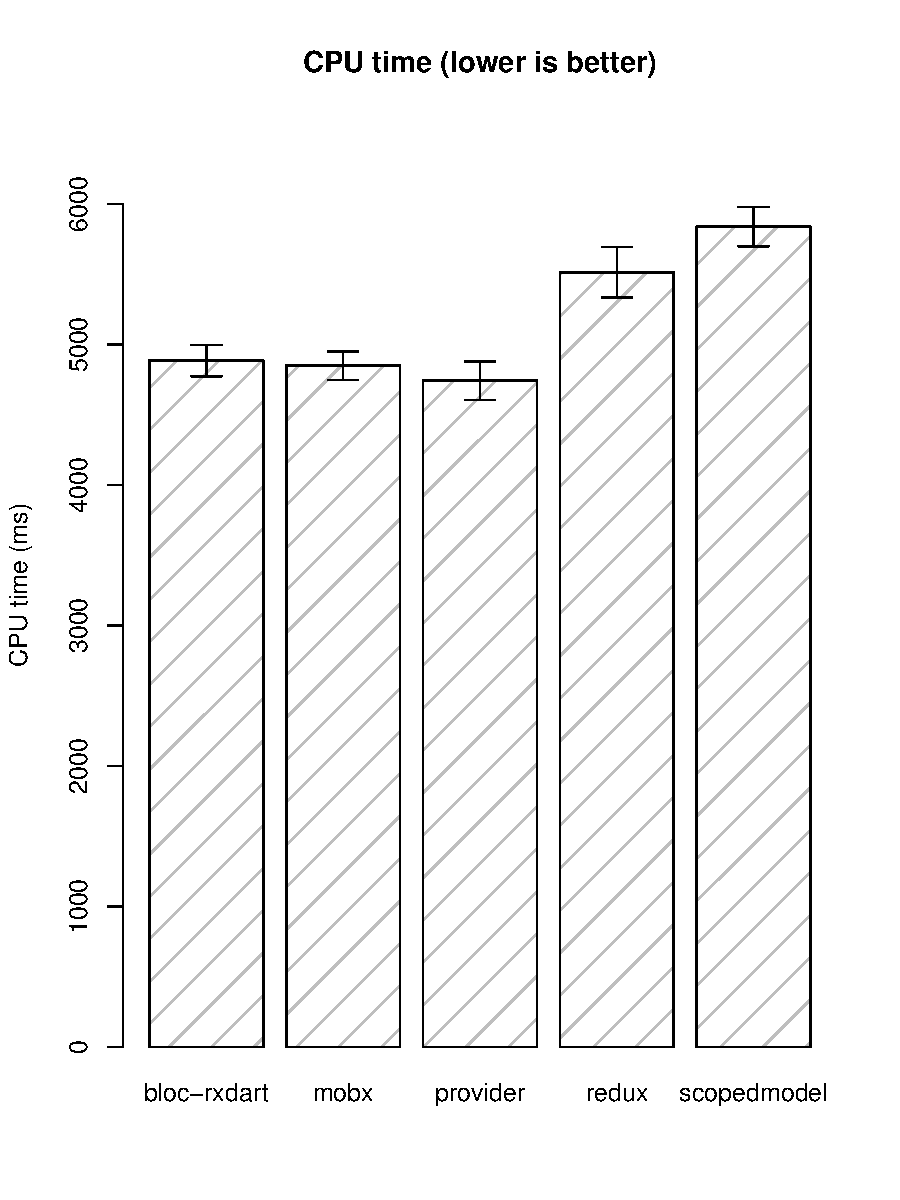
\includegraphics[width=0.8\linewidth]{img/experiment/cpu_time.pdf}
    \caption{Grafiek van de CPU-tijd van de verschillende benaderingen}
    \label{fig:graph-cpu-time}
\end{figure}
Dit experiment toont aan dat de Provider State Management benadering over het algemeen resulteert in de beste performantie voor dit experiment. Deze conclusie is gebaseerd op de CPU-tijden en overgeslagen frames. Hieruit kan echter niet geconcludeerd worden dat Provider altijd de beste benadering zal zijn. \newline \newline
Ten eerste is de applicatie in dit experiment geen volledige voorstelling van een applicatie in productie. In de dit experiment wordt enkel rekening gehouden met state in de applicatie, zonder data op te halen van een externe backend. In deze applicatie worden de producten niet opgehaald door middel van een netwerk request, er wordt enkel gebruik gemaakt van gemockte producten. Dit experiment is representatief voor applicaties die enkel gebruik maakt van lokale state. Verder onderzoek moet uitwijzen of de getrokken conclusies gelden voor een applicatie die netwerk requests stuurt. \newline
Het is perfect mogelijk om de netwerk requests te integreren in de State Management van deze applicatie. Dit zal voor enkele benaderingen meer werk vergen dan voor andere. Zo zullen de netwerk requests relatief snel geïntegreerd kunnen worden in de BLoC benadering aangezien deze reeds gebruik maakt van asynchrone streams. \newline \newline
Ten tweede houdt dit experiment enkel rekening met de CPU-tijd en de overgeslagen frames. De data die verworven is   tijdens het doorlopen van de verschillende benaderingen bevat tal van andere maatstaven. Uit deze data werd voor dit onderzoek enkel en alleen gekeken naar de CPU-tijd en de overgeslagen frames, maar het is perfect mogelijk om rekening te houden met meer maatstaven. Zo is het mogelijk om rekening te houden met de build times en de rasterization times. Rasterisation is het concept waarbij een beeld dat bestaat uit vormen wordt omgezet naar een reeks van pixels om zo het gewenste beeld te bekomen. \newline \newline
Ten derde: tijdens het doorlopen van de verschillende benaderingen op het test apparaat werd dit uitgevoerd op een Android toestel. Dit testapparaat behoort tot op heden bij de mid-range smartphones. Er zou getest kunnen worden of gelijkaardige resultaten bekomen worden bij het uitvoeren van dezelfde gebruikersflow bij andere segmenten van de smartphonemarkt. 

Als laatste werd bij dit experiment de gebruikersflow enkel doorlopen op een Android toestel. Het zou interessant zijn, gezien Flutter een cross-platform framework is, om dezelfde gebruikersflow uit te voeren op een iOS testappraat. 

% al de grafieken samen? Tabel?